\documentclass[12pt ,letterpaper]{article}
\usepackage{amsmath}
\usepackage[utf8]{inputenc}
\usepackage{amsfonts}
\usepackage{amssymb}
\usepackage{graphicx}
\usepackage[T1]{fontenc}
%\usepackage[ngerman]{babel}
\usepackage{caption}
\usepackage{refstyle}
\usepackage[left=2cm, right=2cm, top=2cm, bottom=2cm]{geometry}
 
\title{Edwards Biotope - Interdiszipliänres Projekt II}
\date{26.03.2019}

\begin{document}

\maketitle
\tableofcontents
\pagebreak
\section{Abstract}
\section{Einleitung}
\section{Software-Entwicklung}
\subsection{Architektur}
Hier finden sich die Neuerungen zum Thema Architektur


\subsection{Infrastruktur}
Hier finden sich die Neuerungen zum Thema Infrastruktur
\section{Projekt-Management}
\section{Ästhetik} 
\pagebreak
\section{Basics für  \LaTeX}

\subsection{Font-Format}
\emph{Italic} \\
\textbf{Bold} \\
\texttt{Code} \\
Tabstops: Eins \quad Zwei \quad Drei

\subsection{Kommentare}
(siehe Code)
%Kommentare

\subsection{Mathematische Ausdrücke}
Bruch: $\dfrac{a}{b}$ \\
Vektor: $\dbinom{n}{k}$ \\
Wurzel: $\sqrt{2}$ \\
Potenz: $2^{2}$ \\
Summe: $\sum_{n=1}^{\infty} 2^{-n} = 1$ \\
Limes: $\lim_{x\to\infty} f(x)$

\subsection{Bilder}
\begin{figure}[h]
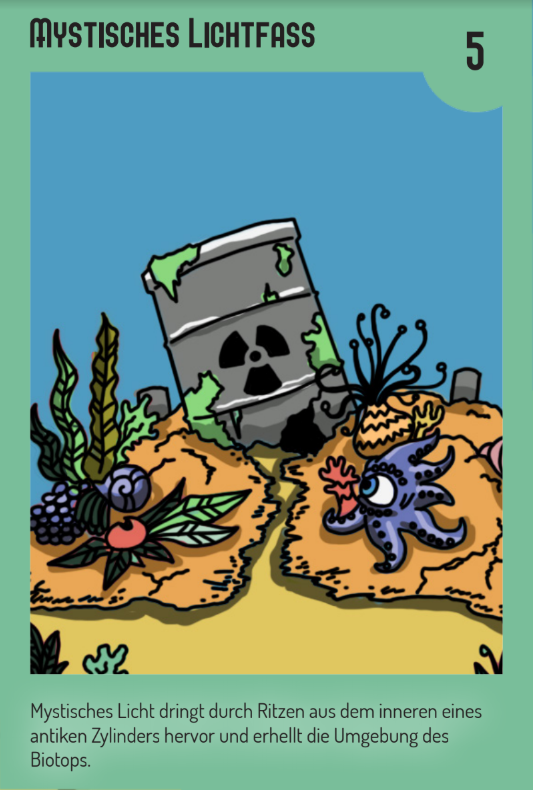
\includegraphics[width=0.2\textwidth]{../img/demo_img.PNG}
\caption{Mystisches Lichtfass}
\label{fig:mystisches_lichtfass}
\end{figure}
Und so referenziert man dynamisch auf die Abbildung \figref{mystisches_lichtfass}

\subsection{Zitate und Referenzen}
So zitiert man mit Referenz \cite[Seite 100]{Test1}


\pagebreak
\begin{thebibliography}{9}
\bibitem{Test1}
Autor, Test,
Ort,
2nd Edition,
2019
\end{thebibliography}

\end{document}